\documentclass[a4paper,12pt]{article}
\usepackage{graphicx}
\usepackage{float}
\usepackage{geometry}
\geometry{margin=1in}

\begin{document}

% University Logo
\begin{center}
    
\includegraphics[width=0.3\textwidth]{images/university.png}  % Replace with your university logo filename
    \\[10pt]
    \textbf{\LARGE VMWare ESXi and VCenter Server Setup}\\[10pt]
    \textbf{Priyanshu Kumar Sharma, B.Tech - CTIS, Sem-6, Sec-B}\\[5pt]
    \textbf{Batch 2022-26}\\[5pt]
    \textbf{Submission Date: 13/03/2025}
\end{center}

\section{Introduction}
Virtualization is a foundational technology that allows multiple operating systems and applications to run on a single physical machine. This report covers the implementation of a virtualization environment using VMware ESXi and vCenter Server.

\section{Objectives}
\begin{itemize}
    \item Understanding VMware virtualization and hypervisor concepts.
    \item Setting up and managing a virtualized infrastructure.
    \item Implementing networking and storage in a virtual environment.
    \item Ensuring security and performance monitoring in VMware.
\end{itemize}

\section{Step-by-Step Implementation}

\subsection{Creating a Virtual Machine using VMware Workstation (Type-2 Hypervisor)}
\begin{enumerate}
    \item Launch VMware Workstation and click \textbf{Create a New Virtual Machine}.
    \item Select \textbf{Typical (recommended)} and click \textbf{Next}.
    \item Choose \textbf{Installer disc image file (ISO)} and select the OS ISO file.
    \item Configure VM settings such as CPU, memory, and disk size.
    \item Click \textbf{Finish} to create the VM.
\end{enumerate}
\begin{figure}[H]
    \centering
    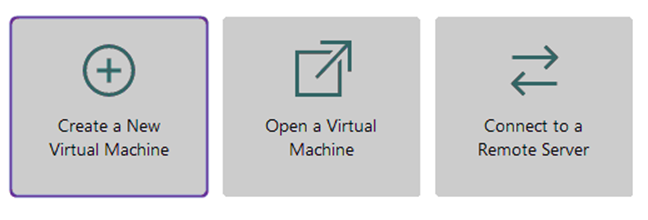
\includegraphics[width=0.8\textwidth]{images/vmware_workstation_setup.png}  % Replace with actual screenshot filename
    \caption{VM Creation in VMware Workstation}
\end{figure}

\begin{figure}[H]
    \centering
    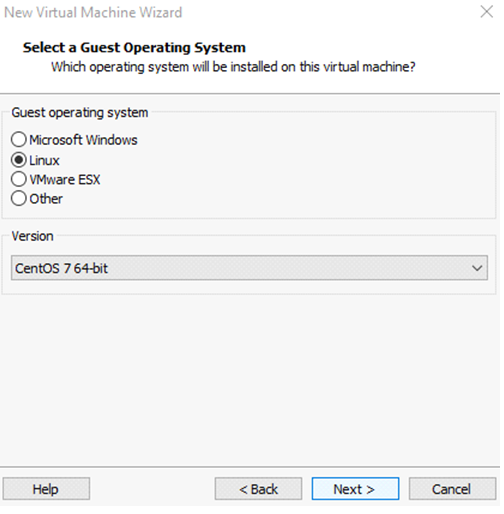
\includegraphics[width=0.8\textwidth]{images/guest_os.png}  % Replace with actual screenshot filename
    \caption{Selecting Operating System}
\end{figure}

\begin{figure}[H]
    \centering
    \includegraphics[width=0.8\textwidth]{ima}  % Replace with actual screenshot filename
    \caption{Final Setup Config}
\end{figure}

\subsection{Practical No. 3: Network Configuration in VMware}

\subsubsection{Adding a Network Adapter}
\begin{enumerate}
    \item Click \textbf{Add > Network Adapter} to add a second network adapter.
    \item Select different networks for ESXi host connections:
    \begin{itemize}
        \item \textbf{NAT Network}: Allows VMs to communicate with the host and access external networks.
        \item \textbf{Host-Only Network}: Allows VMs to communicate only with each other and the host, but not external networks.
    \end{itemize}
\end{enumerate}

\begin{figure}[H]
    \centering
    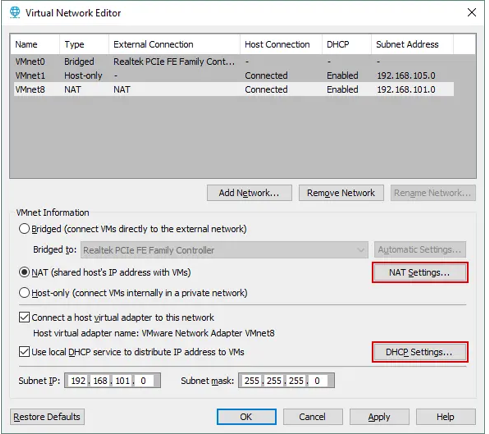
\includegraphics[width=0.8\textwidth]{images/adapter_config.png}  % Replace with actual screenshot filename
    \caption{Adding a Network Adapter}
\end{figure}

\subsubsection{Editing the Virtual Network Configuration}
\begin{enumerate}
    \item Open the \textbf{Virtual Network Editor} (\textbf{Edit > Virtual Network Editor}).
    \item Configure the following networks:
    \begin{itemize}
        \item \textbf{VMnet8 (NAT network)}
        \begin{itemize}
            \item Network Address: 192.168.101.0/24
            \item Gateway IP: 192.168.101.2
            \item DHCP Range: 192.168.101.201 – 192.168.101.254
        \end{itemize}
        \item \textbf{VMnet1 (Host-Only network)}
        \begin{itemize}
            \item Network Address: 192.168.105.0/24
            \item DHCP Range: 192.168.105.201 – 192.168.105.254
        \end{itemize}
    \end{itemize}
    \item Adjust NAT settings, gateway IP, and DHCP configurations as needed.
\end{enumerate}
\begin{figure}[H]
    \centering
    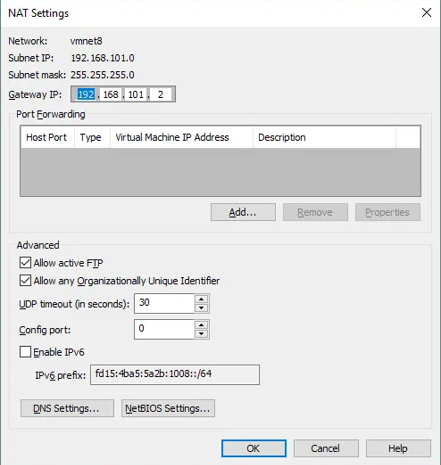
\includegraphics[width=0.8\textwidth]{images/dhcp_config.png}  % Replace with actual screenshot filename
    \caption{Configuring DHCP}
\end{figure}

\begin{figure}[H]
    \centering
    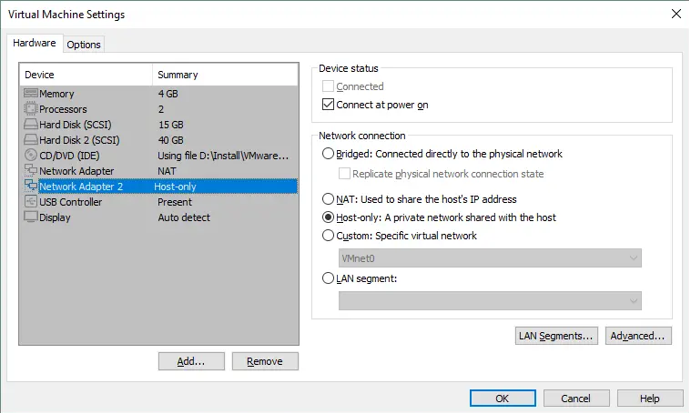
\includegraphics[width=0.8\textwidth]{images/network_adapter.png}  % Replace with actual screenshot filename
    \caption{Editing the Virtual Network Configuration}
\end{figure}



\subsubsection{Basic ESXi Configuration}
\begin{enumerate}
    \item Power on the ESXi VM and press \textbf{F2} to customize the system.
    \item Navigate to \textbf{Configure Management Network}.
    \item Select \textbf{Network Adapters} to view available adapters.
    \item Enable the second adapter later through the web interface.
    \item Set a static IPv4 address:
    \begin{itemize}
        \item IPv4 Address: 192.168.101.101
        \item Subnet Mask: 255.255.255.0
        \item Default Gateway: 192.168.101.2
    \end{itemize}
\end{enumerate}
\begin{figure}[H]
    \centering
    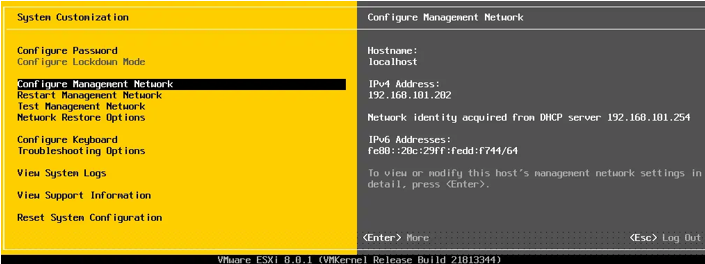
\includegraphics[width=0.8\textwidth]{images/Configure Management Network.png}  % Replace with actual screenshot filename
    \caption{Configuring ESXi Network Settings}
\end{figure}

\section{Conclusion}
This project successfully implemented a virtualization environment using VMware ESXi and vCenter Server. Future improvements could include integrating VMware NSX for advanced networking and automating deployments using vSphere PowerCLI.

\end{document}
